%%%% ijcai22.tex

\typeout{IJCAI--22 Instructions for Authors}

% These are the instructions for authors for IJCAI-22.

\documentclass{article}
\pdfpagewidth=8.5in
\pdfpageheight=11in
% The file ijcai22.sty is NOT the same as previous years'
\usepackage{ijcai22}

% Use the postscript times font!
\usepackage{times}
\usepackage{soul}
\usepackage{url}
\usepackage[hidelinks]{hyperref}
\usepackage[utf8]{inputenc}
\usepackage[small]{caption}
\usepackage{graphicx}
\usepackage{amsmath}
\usepackage{amsthm}
\usepackage{booktabs}
% \usepackage{algorithm}
\usepackage{algorithmic}
\urlstyle{same}

% the following package is optional:
\usepackage{latexsym}

% See https://www.overleaf.com/learn/latex/theorems_and_proofs
% for a nice explanation of how to define new theorems, but keep
% in mind that the amsthm package is already included in this
% template and that you must *not* alter the styling.
\newtheorem{example}{Example}
\newtheorem{theorem}{Theorem}

% Following comment is from ijcai97-submit.tex:
% The preparation of these files was supported by Schlumberger Palo Alto
% Research, AT\&T Bell Laboratories, and Morgan Kaufmann Publishers.
% Shirley Jowell, of Morgan Kaufmann Publishers, and Peter F.
% Patel-Schneider, of AT\&T Bell Laboratories collaborated on their
% preparation.

% These instructions can be modified and used in other conferences as long
% as credit to the authors and supporting agencies is retained, this notice
% is not changed, and further modification or reuse is not restricted.
% Neither Shirley Jowell nor Peter F. Patel-Schneider can be listed as
% contacts for providing assistance without their prior permission.

% To use for other conferences, change references to files and the
% conference appropriate and use other authors, contacts, publishers, and
% organizations.
% Also change the deadline and address for returning papers and the length and
% page charge instructions.
% Put where the files are available in the appropriate places.

% PDF Info Is REQUIRED.
% Please **do not** include Title and Author information
\pdfinfo{
/TemplateVersion (IJCAI.2022.0)
}

\title{Data Corruption Impact on Named Entity Recognition for Low Resourced Languages}

% Single author syntax

\author{
    Anonymous
    \affiliations
    Anonymous
    \emails
    anonymous
}

% Multiple author syntax (remove the single-author syntax above and the \iffalse ... \fi here)
\iffalse
\author{
First Author$^1$
\and
Second Author$^2$\and
Third Author$^{2,3}$\And
Fourth Author$^4$
\affiliations
$^1$First Affiliation\\
$^2$Second Affiliation\\
$^3$Third Affiliation\\
$^4$Fourth Affiliation
\emails
\{first, second\}@example.com,
third@other.example.com,
fourth@example.com
}
\fi

\begin{document}

\maketitle

\begin{abstract}
    African languages have recently been the subject of several studies in Natural Language Processing (NLP) and, this has caused a significant increase in their representation in the field. However, most studies tend to focus more on the models than the quality of the datasets when assessing the models' performance in tasks such as Named Entity Recognition (NER). While this works well in most cases, it does not account for the limitations of doing NLP with low-resource languages, that is, the quality and the quantity of the dataset at our disposal. This paper provides an analysis of the performance of various models based on the quality of the dataset. We evaluate different pre-trained models with respect to the entity density per sentence of some African NER datasets. We hope with this study to improve the way NLP studies are done in the context of low-resourced languages.
\end{abstract}

\section{Introduction}

Africa is one of the most culturally diverse continents in the world. With over 2000 languages spoken on the continent \cite{eberhard_simons_fennig}, we could assume it is the epicentre of the most ground-breaking natural language processing (NLP) researches of the industry. However, this is not the case, as shown in previous studies \cite{nekoto-etal-2020-participatory, Dossou2021CrowdsourcedPT}. The main reason cited is the lack of discoverability of the resources required to conduct such NLP studies \cite{Martinus2019AFO}.

Moreover, considering the case of NER, which is an important subtask of information extraction (IE). Implementing systems that can perform these tasks in the African context could help reduce the communication barrier experienced in some remote parts of the continent, and boost the continent's economy. Therefore, there is a need to improve the representation of African languages in NLP.

Fortunately, some studies made impactful contributions to facilitate future research in NER \cite{10.1162/tacl_a_00416} and other NLP tasks \cite{abs-2104-01443, abs-2103-08647, abs-2103-15963} for African languages. However, they fall short in assessing the performance of these models concerning some limitations faced with low-resource languages. One of them is the difficulty of finding experienced annotators and the high cost of hiring them.

Therefore, our study aims at looking for ways to optimize the cost of hiring annotators in relation to the number of annotations we need to build a decently accurate NLP model. We achieve this by evaluating how the performance of pre-trained models in NER tasks evolves with the availability of annotations in the dataset. We considered NER due to its prevalence in many NLP systems, and we chose pre-trained models to evaluate how prior knowledge of one or more language morphologies could influence the performance of the models. We claim that a linear improvement in the labels' density of a NER dataset does not forcefully produce a linear improvement in the model's performance. As a result, the main contribution of our paper is the analysis of how the quality of low-resourced language data for NER tasks impacts the performance of pre-trained models.

Our work is structured as follows. Section \ref{sec:re} gives a brief overview of the work done in NER. Section \ref{sec:met} gives a thorough description of the approach we followed and, Section \ref{sec:exp} provides the experiments we conducted to validate the claim made in this study. Section \ref{sec:res} provides the results of the experiments conducted and a discussion about the obtained results. Finally, we conclude our work in Section \ref{sec:conc}.

\section{Background}
\label{sec:re}
NER has been an extensively studied NLP task throughout previous years \cite{wang-etal-2019-crossweigh,LampleBSKD16,StrubellVBM17,abs-2105-03654} and, while most studies were done with English corpora, a fair amount of them has also been done with other languages \cite{8700549, abs-2101-01476, Al-RfouKPS14}. But despite the amount of work done, there are relatively few studies in NER about African languages. Nevertheless, due to the contributions of numerous researchers across the continent, NER studies can be conducted using publicly available datasets.

Among those publicly available datasets, we have the MasakhaNER corpus \cite{10.1162/tacl_a_00416}, which includes annotations of sentences for ten spoken African languages and NaijaNER corpus \cite{abs-2105-00810}, restricted to five Nigerian languages. In addition to those datasets, we have SADiLaR \cite{eiselen-2016-government} for ten of the official South African languages and, though datasets play a crucial role in every NLP system, we cannot neglect the part played by the models trained on these data.

From rule-based systems like FASTUS \cite{appelt-etal-1995-sri} to deep learning models \cite{abs-1812-09449}, NER has evolved into a data-centric task. In between this evolution, many NER techniques were proposed. Among some of them, we have sequence labelling methods such as Conditional random fields (CRFs), which models the conditional probability over label sequences given a sequence of observations. Examples of CRFs for NER includes Bi-LSTM-CRF \cite{HuangXY15}, CNN-LSTM-CRF \cite{abs-1905-01964} and BERT-CRF \cite{abs-1909-10649}. Other NER systems use Hidden Markov Models (HMMs) to identify entities in a corpus \cite{10.1007/978-3-540-77046-6_67}. The use of HMMs is motivated by their reliability to analyse sequential correlations between neighbouring samples, notably texts data.

However, the biggest breakthrough in NER and other NLP tasks came from the use of large pre-trained languages models such as BERT  \cite{abs-1810-04805}, RoBERTa \cite{abs-1907-11692} and, GPT-3 \cite{abs-2005-14165}, and while these language models mainly differ by the number of parameters they possess, they are capable of achieving state-of-the-art results in various NLP tasks. The majority of these language models are trained on English corpora but, there exist some variants trained on other languages \cite{abs-1911-03894, abs-2012-02110, CaneteCFP2020} as well as others trained on more than one language. This is the case for mBERT \cite{abs-1911-03310} trained on 104 languages and XLM-RoBERa \cite{abs-1901-07291} trained on 100 languages.

\section{Methodology}
\label{sec:met}

In this section, we introduce the different components that permit us to carry out this study. Firstly, we talk about the dataset used in this study. Secondly, we provide a detailed list of models used as well as the reason behind each choice. Lastly, we speak about the evaluation metric used in this study.

\subsection{NER Dataset}

For this study, we use a subset of the MasakhaNER dataset \cite{10.1162/tacl_a_00416}. This dataset consists of corpora from different sources and written in 10 spoken African languages, annotated with entities inspired from English CoNLL-2003 dataset \cite{tjong-kim-sang-2002-introduction}. For each language, there is an annotated corpus divided into three sections: training, development, and testing, which amount to 70\%, 10\%, and 20\% of the corpus, respectively. For this study, we chose to work on 3 languages, namely \textbf{Swahili}, \textbf{Nigerian-Pidgin} and \textbf{Kinyarwanda}. We selected the corpus of these languages based on the number of entities and the percentage of tokens that were named entities. By picking corpora with high entity density, we can vary this density throughout a wide range to see how our models are affected.

\subsection{Models}
To evaluate the performance of our datasets with different entity densities, we use four popular pre-trained models, namely, BERT, RoBERTa, two versions of multilingual BERT
(mBERT). All these models are available through the HuggingFace transformers library \cite{abs-1910-03771}. Half of these models are multilingual. We hypothesize that knowledge of different language morphologies can help in situations where the NER entities are scarce. So, in theory, multilingual models will work better than monolingual ones as the entity density in the training corpus reduces. We only use mBERT due to the limitations in computational resources which does permit us to train larger models such as XLM-RoBERTa.

\subsubsection*{BERT} was proposed as a pre-trained model which could get the bidirectional representation from unlabelled texts \cite{abs-1810-04805}. We fine-tune our model on our corpus for sequence labelling. We use the BERT-base cased model trained on English text with 12 layers of transformers block with a hidden size of 768, 12 attention heads and 110 parameters.

\subsubsection*{RoBERTa} is an optimized version of BERT that outperforms its predecessor \cite{abs-1907-11692}. Through the modifications of some training parameters and an increase in the size of the training data. This version of BERT could achieve state-of-the-art results on popular benchmarks such as n GLUE, RACE and SQuAD. We use the RoBERTa-base model with the same architecture as BERT.

\subsubsection*{mBERT} is the fine-tuned version of BERT, trained on 104 languages \cite{abs-1911-03310} (Swahili included). We fine-tune two cased versions of this model with the same architecture as BERT. However, this model has 179M parameters. The first version is trained on 104 languages through masked-language modelling, and the second one is a fine-tuned version of the first on 10 high resourced languages for NER tasks. We hypothesize that the second version will outperform the first one due to the focus of its training objective towards NER.

% \subsubsection*{XLM} was introduced with a new method of learning cross-lingual language representation called Translation Language Modelling (TLM) \cite{abs-1901-07291}. The TLM approach is an extension of Masked Language Modelling (MLM). However, TLM differs from MLM by using multiple language translations of the same sentence to predict the masked word. We use a version of XLM, trained with 100 languages. This version possesses 16 layers of transformers block with a hidden size of 1280, 16 attention heads.%

\subsection{Evaluation Metrics}
We evaluate the performance of different models using the F1-score metrics. The formula is given by:

$$F1 = \frac{\mathrm{TP}}{\mathrm{TP}+\frac{1}{2}(\mathrm{FP}+\mathrm{FN})}$$

where $\mathrm{TP}$, $\mathrm{FP}$, $\mathrm{FN}$, $\mathrm{TN}$ represents the true positives, false positives, false negatives and true negatives of the model's prediction.

\section{Experimental Setup}
\label{sec:exp}
Throughout this section, we thoroughly explain how we plan to evaluate the performance of pre-trained models based on quality. Firstly, we describe the method used to vary the quality of the dataset and lastly, we will explain how we plan to evaluate the performance of different models holistically.

% and through a bucket-based approach.

\subsection{Varying the Quality of the Dataset}
\label{sec:exp:var}
Our main claim in this study is to show that a linear improvement in the dataset's quality does not forcefully produce a linear improvement in the performance of the model. Therefore, we need a method to vary the quality of the dataset linearly. For that, we must first explain what we mean by the quality of the dataset. In this study, the dataset's quality is the number of entity labels per sentence in the NER corpus. So, varying this quality means modifying this attribute for every sentence in the datasets corpus. We do this by creating buckets where we threshold this attribute over a specific range. In other words, we build buckets of the same dataset in which each sentence in the corpus have at most \textit{n} entity label with n being the threshold that characterizes the bucket.

\begin{figure}
    \centering
    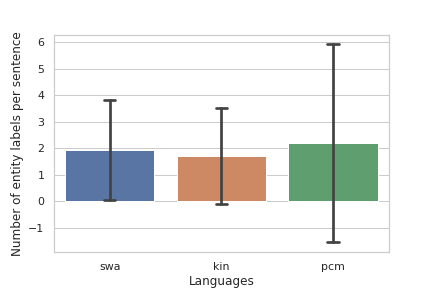
\includegraphics[width=\columnwidth]{images/dist_plot.png}
    \caption{Distribution of entity labels per sentence for three language namely, Swahili (swa), Kriyananda (Kin) and Nigeria-Pidgin (pcm). The error bar represents the standard deviation}
    \label{fig:dist}
\end{figure}

\begin{figure}
    \centering
    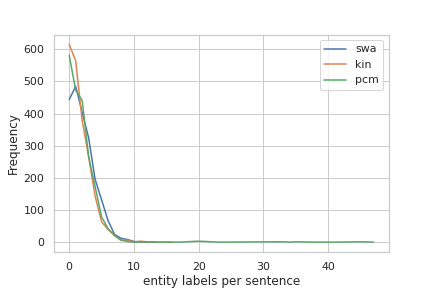
\includegraphics[width=\columnwidth]{images/evlution.png}
    \caption{A plot of the frequency at which a sentence has a particular number of entity labels for three languages, Swahili (swa), Kriyananda (Kin) and Nigeria-Pidgin (pcm).}
    \label{fig:evolution}
\end{figure}

We see from Figure \ref{fig:evolution} that the Nigerian corpus has the most diverse corpus in terms of the number of entities in a single sentence. Additionally, we see from Figure \ref{fig:dist} that the number of sentences with entity labels in the range [1 - 10] is more frequent than sentences with this attribute in any other range. For this reason, bucketing training data with the number of entity labels varying along this range will suffice to get meaningful results.

\subsection{Holistic Evaluation}
This evaluation's method consists of evaluating the performance of each model on the overall quality of our dataset. We perform this with the model and the uncapped version of the dataset used to train the model. This method does not differ from the usual way of evaluating models in research papers.

% However, this method does not give insights on how our model performance in various scenarios. 

%This is why we also carry a \textit{bucket-base evaluation} on the models and datasets.

%\subsection{Bucket-Based Evaluation}
%Bucket-based evaluation permits us to identify the strength and weaknesses of our models on various aspects of our datasets. For this evaluation, we segment our dataset into several buckets and evaluate our models on each bucket. Here, we bucket the evaluation dataset the same way as we did with the training set and we available models trained on sentences with different entity cap, on test data with different entity cap. We hypothesize that models trained with buckets at an entity cap k will have a hard time with sentences with more entities.

\section{Results and Analysis}
\label{sec:res}
%\subsection{Holistic results}

\begin{figure}
    \centering
    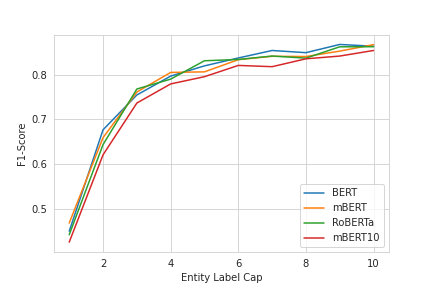
\includegraphics[width=\columnwidth]{images/pcm_models_plot.png}
    \caption{A plot of the F1-score against the entity label cap for all sentences of the Nigerian Pidgin corpus (pcm).}
    \label{fig:pcm_plot}
\end{figure}

\begin{figure}
    \centering
    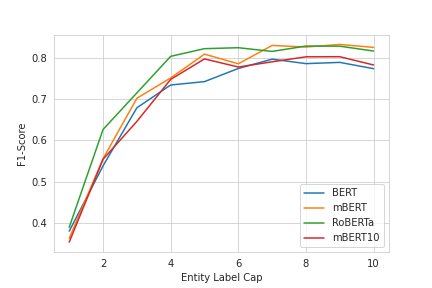
\includegraphics[width=\columnwidth]{images/kin_models_plot.png}
    \caption{A plot of the F1-score against the entity label cap for all sentences of the Kinyarwanda corpus (kin).}
    \label{fig:kin_plot}
\end{figure}

\begin{figure}
    \centering
    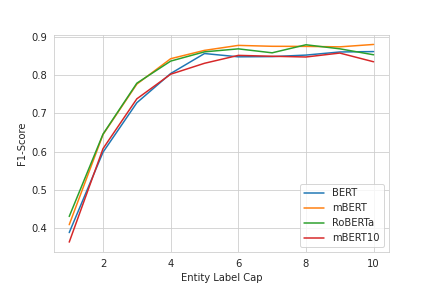
\includegraphics[width=\columnwidth]{images/swa_models_plot.png}
    \caption{A plot of the F1-score against the entity label cap for all sentences of the Swahili corpus (swa).}
    \label{fig:swa_plot}
\end{figure}

\begin{table*}
    \small
    \centering
    \label{UNET_and_GMM}
    \begin{tabular}{cccc}
        \toprule
        Models      & Kinyarwanda    & Nigerian Pidgin & Swahili        \\  \midrule
        BERT-c1     & 37.95          & 44.97           & 38.72          \\
        BERT-c5     & 74.32          & 81.95           & 85.74          \\
        BERT-c10    & \textbf{77.46} & \textbf{86.33}  & \textbf{86.25} \\ \midrule
        mBERT-c1    & 36.19          & 46.81           & 40.8           \\
        mBERT-c5    & 81.0           & 80.61           & 86.56          \\
        mBERT-c10   & \textbf{82.64} & \textbf{86.69}  & \textbf{88.12} \\ \midrule
        RoBERTa-c1  & 38.9           & 44.19           & 42.95          \\
        RoBERTa-c5  & \textbf{82.33} & 83.09           & \textbf{86.18} \\
        RoBERTa-c10 & 81.75          & \textbf{86.23}  & 85.41          \\ \midrule
        mBERT10-c1  & 35.28          & 42.54           & 36.22          \\
        mBERT10-c5  & \textbf{79.84} & 79.53           & 83.17          \\
        mBERT10-c10 & 78.36          & \textbf{85.39}  & \textbf{83.57} \\
        \bottomrule
    \end{tabular}
    \caption{Performance of each model for Entity Label Cap ${1, 5, 10}$ for every language. (1) The name of model followed by \textbf{-c5} indicates that this model has been trained on training data with \textit{Entity Label Cap} = 5. Example: BERT-c10 means that the BERT model was trained on training data with \textit{Entity Label Cap} = 10. (2) mBERT10 is the fine-tuned version of mBERT on 10 high resourced languages, specifically of NER}
\end{table*}

In this evaluation, we trained and evaluated our models with datasets with 10 entity cap values. For each cap value $j = \{1,2, \dots, 10\}$, we created a corpus where we cut off (transform to \textit{O} token) the labels of the sentences which had more than j entities and, we trained and evaluated our models with the processed corpus. From figures \ref{fig:swa_plot}, \ref{fig:kin_plot} and \ref{fig:pcm_plot}, we see that the performance of our models does not differ much. It indicates that multilingual models do not bring any significant benefit for this task. This may be because all low-resourced African languages, except Swahili, used in this study, were not part of the languages used to train these large multilingual models. Also, this can explain why the performance of models in the Swahili corpus at Figure \ref{fig:swa_plot} seems to be the best.

The original claim of this study was that a linear improvement in the labels' density of a NER dataset does not forcefully produce a linear improvement in the model's performance. We can confirm this by looking at the plot in figures \ref{fig:swa_plot}, \ref{fig:kin_plot} and \ref{fig:pcm_plot}. We observe that while there is a steady increase in the performance of our model as we increase the entity cap, the curve starts to flatten down around \textit{Entity Label Cap} = 6. This indicates that as we had more sentences to labels after this cap, there was not much performance improvement on the models (both monolingual and multilingual).

\section{Impact Statement}
Analyzing the performance of NER models in the way we did gives us some knowledge of how many resources we need to construct NER corpora. In this way, we would build datasets with just enough labels to get good models' performances and maximize the return per investment on the dataset creations.

Also, there are many benefits in carrying such studies. In the African context, NLP is still an undervalued field and scarcity of resources makes it hard to create an ecosystem in which this field can evolve. A direct consequence is the difficulty to find good annotators for African datasets' creation. Our research cements the idea that the quality of a NER dataset mostly depends on the corpus itself and, more labels do not always equate to better performance. It can help us budget the cost of datasets creation efficiently. However, there are some drawbacks with this type of analysis: (i) It requires enormous training of our models with different instances of the same dataset. Our study, for example, trained 4 models for 3 languages using 10 different entity caps. It makes a total of 120 training experiments. In the long run, this will have negative effects on the environment. (ii) In addition, such studies, which require such a large amount of resources, cannot be carried out in the African context without consequent funding.

There is a possibility to do similar analyses with several African languages and other NLP tasks such as text classification. One example would be a study that trains models on different corpora with different levels of grammatical errors. The results obtained from that study could help us get insights into how corpus from unsupervised training corpus influences our models in terms of its performance and fairness.

% \subsection{Bucket-based results}
\section{Conclusion}
\label{sec:conc}

In this study, we claimed that a linear improvement in the density of labels in the model does produce a linear improvement in the performance of pre-trained language models in the context of low-resourced NER tasks. This claim was verified by training different models on low-resource African language NER corpora and at different levels of density labels. After a certain level of entity cap, each model's performance stagnates. This behaviour was consistent across all the language corpora used to train our models.

Our study proves that we do not forcefully need to build a highly dense NER corpus to produce good models performance. We hope by this work to encourage dataset creators for NLP tasks to privilege the curation of their corpus over the density of the label present in these corpora. Finally, a future improvement could be to use more models to see if this behaviour replicates and extend this type of analysis for other NLP tasks.

%% The file named.bst is a bibliography style file for BibTeX 0.99c
\bibliographystyle{named}
\bibliography{ijcai22}

\end{document}

